\chapter{Introduction}
The Standard Model of particle physic has enjoyed an unprecedented level of success since its completion in the late 1960s. Together with Einstein's theory of general relativity, today's physicists possess the ability to understand Nature on both the smallest and largest of scales.

The legacy of the Standard Model has been bolstered in recent years by a number of experimental achievements. The discovery of the Higgs boson by the ATLAS \cite{the_atlas_collaboration_observation_2012} and CMS \cite{the_cms_collaboration_observation_2012} teams at the Large Hadron Collider in the summer of 2012 completed the Standard Model's last missing link. Further analyses by ATLAS and CMS have since confirmed that the discovered Higgs boson has exactly the predicted properties and couplings to other particles. The discovery of gravitational waves in 2015 by the LIGO experiment \cite{ligo_scientific_collaboration_and_virgo_collaboration_observation_2016} provided spectacular confirmation of one of the most intriguing predictions of general relativity. Our understanding of the Universe has never been on such sure footing.

And yet for all its successes, the Standard Model remains, at best, frustratingly incomplete. Astronomical observations indicate the presence of large amounts of dark matter, whose energy density dwarfs that of the known Standard Model components. Although no experiment to date has seen significant deviations from the predictions of general relativity or the Standard Model, the two theories are also known to be incompatible on a fundamental level. With careful experimentation, physicists can study these problems head-on, and perhaps make progress towards addressing them. 

\section{Dark Matter}
Multiple lines of inquiry have firmly established that a majority of the energy density of the Universe is composed of a component which is neither baryonic nor luminous. The first indications of what we now call dark matter (DM) were Zwicky's observations in 1933 that the velocity dispersion of galaxies in the Coma Cluster was far higher than the escape velocity predicted from the mass of the luminous galaxies \cite{zwicky_1933}. Later observations of galaxy clustering, for example Kahn \& Woltjer's analysis of the motion of Andromeda \cite{kahn_intergalactic_1959}, further indicated that galaxies were far more massive than conventionally expected. Evidence continued to mount in the 1970s as work done by Rubin \& Ford \cite{rubin_rotation_1970} and Roberts \& Rots \cite{roberts_comparison_1973} showed that the rotation curve of Andromeda was flat out to large distances (30 kpc) from the galactic center, indicating that the mass-to-light ratio at large radii was far larger than that of a typical star. Further data from Rubin \cite{rubin_extended_1978} subsequently confirmed that the same result held true for a nearly all spiral galaxies she considered. 
 
The mystery deepened as it became clear that the dark matter could not be composed of traditional baryonic matter. The most visceral indication of this comes from a comparison of the gravitational lensing by merging galaxies in the Bullet Cluster to an X-ray tracer of the gas content \cite{clowe_direct_2006}, as seen in Figure \ref{fig:clowe}. The data shows conclusively that although the gas dominates the visible mass of the cluster, the lion's share of the mass undergoes little self-interaction. Moreover, Big Bang nucleosynthesis (BBN) constrains the baryonic density of the the Universe to be less than about one twentieth of the critical density $\Omega_c$, but the astronomical observations indicate that the DM density is approximately a quarter of the critical density. Finally, the scale of temperature fluctuations in the CMB is too small to account for the observed density clustering in today's Universe, but the problem can be resolved if the Universe has a large nonbaryonic component \cite{einasto_dark_2009}.

\begin{figure}
\begin{center}
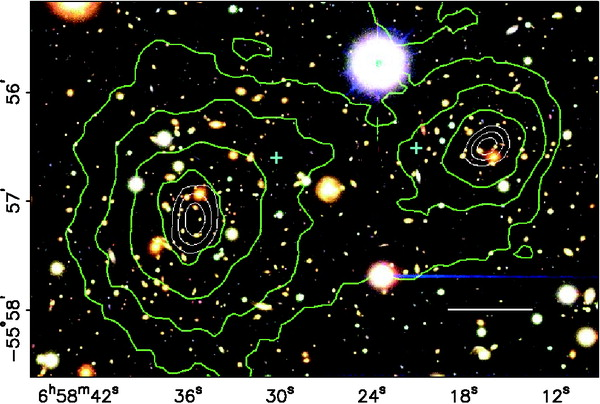
\includegraphics[width=0.45\columnwidth]{figures/clowe_a.jpg}
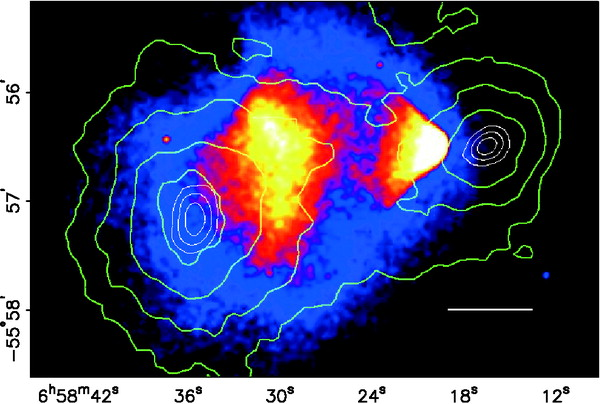
\includegraphics[width=0.45\columnwidth]{figures/clowe_b.jpg}
\end{center}
\caption{
\label{fig:clowe}
{\it Left panel:} Optical image of the colliding Bullet cluster, taken with the Magellan telescope.
{\it Right panel:} X-ray image of the same region from the Chandra space telescope.
In both panels, the white contours show the location of the region of maximum gravitational shear.
The gas content, traced by the X-ray emission, lags behind the bulk of the mass due to scattering during the collision.
Figure reproduced from \cite{clowe_direct_2006}.
}
\end{figure}


Today, DM plays a key role in the successful $\Lambda$CDM model of the Universe by seeding density fluctuations around which galaxies grow.
N-body simulations of galaxy formation with cold dark matter have shown great success at reproducing the observed structure \cite{bertone_particle_2010}.
The exact nature of the DM, however, remains unkown.
The known massive neutral particles in the Standard Model (e.g. the Higgs or Z bosons, the neutron) all decay too quickly to account for the presence of DM at the current time. Of the remaining neutral particles, the only plausible candidates are the neutrinos, but their low mass precludes them from moving slowly enough to form structures as small as galaxies \cite{einasto_dark_2009}. 

A variety of candidates for the identity of dark matter have been proposed, most of which require extensions to the Standard Model. 
These extensions invariably predict the existence of new neutral, stable particles, of which the most widely studied are axions and WIMPs.

\subsection{Axions}
The motivation for axions comes from the strong CP problem- the question of why CP (charge \& parity) symmetry is conserved to a high degree in the strong interaction despite the O(1) CP-violating phase in the weak interaction. Assuming the Universe is not fine-tuned, CP violation in QCD can be made small dynamically by the introduction of a new U(1) symmetry (the Peccei-Quinn symmetry). The Nambu-Goldstone bosons of this new symmetry are the axions, in much the same way as the photon is the Goldstone boson of the U(1) symmetry associated with the electromagnetic interaction. 
If they exist, axions must have extremely small masses and low couplings to Standard Model particles. Constraints from beam-dump experiments and astrophysical searches require the axion mass to be less than approximately $10^{-3}$ eV. On the other hand, the axion mass must be greater than approximately $10^{-6}$ eV in order to not overclose the Universe \cite{bertone_particle_2010}. If the axion mass is near its lower bound, axions are a plausible DM candidate. Although lighter than neutrinos, the density fluctuations in the axion field are localized enough to reproduce the DM substructure that we observe. A variety of experiments to search for axions are underway, which generally seek to excite the axion field and produce resonant photons via the Primakoff process. 

\subsection{WIMPs}
Weakly Interacting Massive Particles (WIMPs) are a class of particle which generally possess masses and coupling strengths on the order of the electroweak scale (roughly 100 GeV). 
Such particles would have been in thermal equilibrium with the rest of matter at moments shortly after the Big Bang.
However, as the Universe expanded and cooled, WIMPs would have fallen out of equilibrium when the Hubble rate exceeded the WIMP-SM interaction rate. 
As it turns out, a weak-scale cross-section yields dark matter that "freezes out" from the rest of the Universe at precisely the correct time to yield the observed relic abundance, a coincidence which has been dubbed the 'WIMP miracle' \cite{bertone_particle_2010}.

Generally speaking, there are three paradigms through which to search for WIMP dark matter.
WIMPs can be produced in collisions at high-energy particle accelerators like the LHC.
In this case, the stable and neutral WIMPs will escape the detector apparatus, leading to "missing" transverse momentum in the reconstructed final state of particles.
Such searches must contend with significant backgrounds from SM electroweak processes which produce neutrinos.
The scattering of WIMPs off of nucleons can also be searched for by low-background counting experiments.
These experiments are typically performed deep underground to avoid contamination by showers from cosmic rays.
Finally, WIMPs may annihilate or decay to Standard Model particles, which can be detected by looking at areas in the Universe where high concentrations of dark matter exists are believed to exist.
Searching for WIMP annihilation via this 'indirect detection' paradigm will be the focus of Chapters \ref{chapter:pwave} \& Y\ref{chapter:pwave_analysis}. 

\subsection{PBHs}
Unlike many other dark matter candidates, primordial black holes (PBHs) are attractive as dark matter candidates because they require little new physics beyond the Standard Model.
Producing enough PBHs to account for the present DM density is subject to some theoretical difficulties, but several authors have argued that they could arise naturally in a variety of scenarios (see Section X for more details).
PBHs also present straightforward detection strategies- heavy PBHs can in principle be detected via the gravitational wave events from their mergers; intermediate-mass PBHs can be constrained by their accretion onto neutron stars and white dwarfs \cite{pani_tidal_2014} or potentially detected via microlensing events \cite{carr_primordial_2016}. Low-mass PBHs can be detected by their Hawking radiation; a more detailed discussion of PBHs as dark matter candidates and the prospects for detecting low-mass PBHs will follow in Section \ref{chapter:pbhs}. 

\section{Quantum Field Theory in Curved Spacetime}
Although general relativity and the Standard Model excel at describing Nature on large and small scales, respectively, a complete theory of quantum gravity remains unknown. Theorists have had some success (see the results in Section X, for instance) in describing quantum field theories in a background of curved spacetime, but generally these models neglect perturbative interactions in favor of free fields. 
As noted in Wald \cite{wald_general_1984}, the source of the difficulty in constructing a completely satisfactory theory of quantum gravity is rooted in the fact that the metric $g_{\mu\nu}$ is both the dynamical variable of general relativity and the description of the spacetime in which the quantum theory lives.
Attempts to construct perturbative theories of gravitation via Einstein's equation for a massless spin-2 field have therefore failed, usually due to the fact that these theories are generally nonrenormalizable.

In the face of these theoretical challenges, unfortunately, experiments also offer little guidance.
The problem for experimentalists is essentially one of mismatched scales: gravitation is extraordinarily weak on the scale of a typical quantum system.
A rough sense of the mismatch is given by the fact that Newton's gravitational constant is approximately 42 orders of magnitude weaker than the Coulomb constant.
The Planck scale (roughly $10^{18}$ GeV), where GR effects become important in quantum systems, is far beyond the reach of even the most ambitious particle accelerator designs.
Only a handful of instances exist where general relativity can conceivably be applied to a quantum system- the Big Bang, for instance.
Observing the Big Bang directly in the electromagnetic spectrum is made difficult by the presence of the cosmic microwave background (CMB).
Future experiments, however, may be able to detect primordial gravitational waves (either directly or via B-mode polarizations in the CMB) that are predicted to arise from models of inflation and thus provide a crucial test of theories of the Big Bang.
Alternatively, PBHs provide a natural laboratory for observing physics at the Planck scale: as PBHs evaporate, their temperature diverges towards the Planck scale and necessarily new physics will describe their dynamics. A search for PBHs in this context is described in Chapters \ref{chapter:pbhs} \& \ref{chapter:pbh_analysis}.

In the work that follows I present two analyses that make use of data from the Fermi Large Area Telescope (Fermi-LAT) to search for evidence of dark matter and PBHs. I will show that the capabilities of {\it{Fermi}}-LAT allow it to test models of physics that cannot be studied with other means. Gamma-ray astrophysics remains one of the best available probes of physics beyond the Standard Model.

